\uuid{SGnO}
\exo7id{5824}
\auteur{rouget}
\organisation{exo7}
\datecreate{2010-10-16}
\isIndication{false}
\isCorrection{true}
\chapitre{Conique}
\sousChapitre{Parabole}

\contenu{
\texte{
Equation cartésienne de la parabole $(\mathcal{P})$ tangente à $(Ox)$ en $(1,0)$ et à $(Oy)$ en $(0,2)$.
}
\reponse{
On cherche une équation sous la forme $(ax+by)^2 + 2cx + 2dy + e = 0$ avec $a^2+b^2 = 1$  et $a > 0$.

\textbullet~$(1,0)\in(\mathcal{P})\Leftrightarrow a^2+2c+e = 0$   et $(0,2)\in(\mathcal{P})\Leftrightarrow4b^2+4d+e=0$.

\textbullet~D'après la règle de dédoublement des termes, la tangente en $(1,0)$ à $(\mathcal{P})$ admet pour équation cartésienne $a^2x +aby+ c(x+1) +dy + e = 0$  ou encore $(a^2+c)x + (ab+d)y + c+e = 0$. Cette tangente est l'axe $(Ox)$ si et seulement si $a^2+c = 0$ et $c+e = 0$ et $ab+d\neq 0$.

\textbullet~La tangente en $(0,2)$ à $(\mathcal{P})$ admet pour équation cartésienne $2abx + 2b^2y + cx + d(y+2) + e = 0$ ou encore $(2ab+c)x + (2b^2+d)y +2d+e = 0$. Cette tangente est l'axe $(Oy)$ si et seulement si $2b^2+d = 0$ et $2d+e = 0$ et $2ab+c\neq 0$.

En résumé, $(\mathcal{P})$ est solution si et seulement si $c=-a^2$, $d = -2b^2$, $e = a^2 = 4b^2$, $a^2+b^2 =1$, $ab+d\neq0$, $2ab+c\neq 0$ et $a > 0$.

$a > 0$, $a^2 = 4b^2$ et $a^2+b^2 =1\Leftrightarrow a =\frac{2}{\sqrt{5}}$ et $b =\pm\frac{1}{\sqrt{5}}$.

Les égalités $a=\frac{2}{\sqrt{5}}$ et $b =\frac{1}{\sqrt{5}}$ fournissent $ab+d =\frac{2}{5}-\frac{2}{5}= 0$ ce qui ne convient pas.

Il reste $a =\frac{2}{\sqrt{5}}$, $b = -\frac{2}{\sqrt{5}}$, $c = -\frac{4}{5}$ , $d= -\frac{2}{5}$  et $e  =\frac{4}{5}$  qui fournit bien une solution. On trouve une et une seule parabole. 

\begin{center}
\shadowbox{
La parabole $(\mathcal{P})$ admet pour équation cartésienne $(2x-y)^2 -8x - 4y + 4 = 0$.
}
\end{center}

$$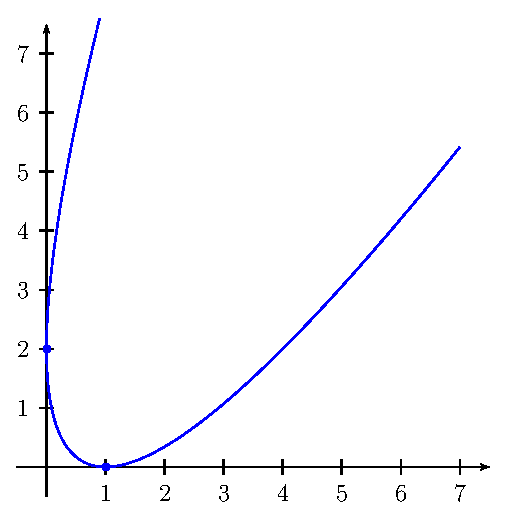
\includegraphics{../images/img005824-1}$$
}
}
